\documentclass[conference]{IEEEtran}
\IEEEoverridecommandlockouts
% The preceding line is only needed to identify funding in the first footnote. If that is unneeded, please comment it out.
\usepackage{cite}
\usepackage{amsmath,amssymb,amsfonts}
\usepackage{algorithmic}
\usepackage{graphicx}
\usepackage{listings}
\usepackage{textcomp}
\usepackage{xcolor}
\usepackage[htt]{hyphenat}
\def\BibTeX{{\rm B\kern-.05em{\sc i\kern-.025em b}\kern-.08em
    T\kern-.1667em\lower.7ex\hbox{E}\kern-.125emX}}
\begin{document}

\title{PentaPico: A Raspberry Pi Pico Based Cluster For Image Convolution Tasks}

\author{\IEEEauthorblockN{1\textsuperscript{st} Willow Cunningham}
\IEEEauthorblockA{\textit{Department of Electrical and Computer Engineering} \\
\textit{University of Maine}\\
Orono, United States \\
willow.e.cunningham@maine.edu}
}

\maketitle

\begin{abstract}
For longer than I have been alive, cluster computers have been the state of the art technology in high performance computing. 
In order to lower the barrier of entry to cluster computing the world of low cost clusters made of single board computers like the Raspberry Pi has been thoroughly explored, but these clusters can still cost hundreds of dollars.
To this day, I believe that the potential of microcontrollers to provide the basis for ultra-cheap cluster computers is underexplored.
In my Cluster Computing project I create a cluster computer out of $5$ Raspberry Pi Picos (Picos) and program the cluster to compute image convolutions using I$^2$C as the inter-node communication protocol.
Unfortunately, I find that slow data rate of I$^2$C completely undermines any attempts to take advantage of algorithmic parallelism with the cluster. 
The results indicate that using all $4$ compute nodes causes a $0.76$x \textit{slowdown}.
\end{abstract}

\section{Introduction}
% What your project is and what the goal was

My project is to create a cluster computer out of Raspberry Pi Pico (Pico) microcontrollers that is capable of computing image convolutions. 
The goal was primarily to see if I personally had the programming skills and knowledge to successfully create a cluster computer using microcontrollers, and secondly to see how viable such clusters are for any practical use case.

In this report, Section~\ref{related_sec} covers some similar projects.
Section~\ref{hardware_sec} describes the hardware in use as well as the design of the PentaPico cluster.
Section~\ref{software_sec} describes the design and implementation of the software for both the client program and the cluster itself.
Section~\ref{results_sec} discusses the performance of the cluster and challenges faced in the project, and Section~\ref{conclusion_sec} concludes the report.

\section{Related Work}
\label{related_sec}
% List and properly cite at least three related projects that did similar work (academic papers would be best, but you can also cite websites and such). Describe how your work differs from the previous work.

There have been other microcontroller cluster computers created by hobbyists in the past.
The PicoCray by Extreme Electronics~\cite{electronics:hackaday}, a 9-Pico cluster communicating over $I^2C$ and configured to compute the Mandelbrot set, is very similar to my work but poorly documented.
The PicoCray communicates data between nodes in packets of $120$ bytes, while my PentaPico simply transmits the entire stream of data in one packet. 
While the PicoCray contains its own display and does not require user input for its program, the PentaPico relies on a USB serial connection to a personal computer for taking input and displaying results.

Bitluni~\cite{bitluni:hackaday} attempts to create a microcontroller cluster out of the $\$0.10$ CH32V003 RISC-V microcontroller, but does not get much further than implementing a blinking LED program.

Henk Verbeek~\cite{verbeek:zapp} creates a parallel computer out of $80$ PIC32MX170F256 microctontrollers.
The cluster is programmed in BASIC, communicates over I$^2$C, and computes fractal images.
Interestingly, Verbeek finds that maximum speedup is achieved by around $12$ nodes in general, and adding more nodes bogs down the cluster in communication overhead.

Sánchez-Cabadas et al.~\cite{sanchez:JPCS} create a $6$ node cluster based on the PIC16F887 microcontroller. 
Like my cluster, they use I$^2$C to communicate between the nodes.
However, they do not investigate the communication overhead of the cluster.


\section{Hardware}
\label{hardware_sec}
% Describe the computing hardware that you run on. Say if it is shared memory, a distributed system, or something else. List the CPU (architecture, type, speed), RAM, and network.

In this section I cover the hardware of the Pico as well as the configuration of the cluster.

\subsection{Raspberry Pi Pico}

The hardware platform for this project is based on the Pico microcontroller, which has an RP2040 processor. 
The relevant hardware information for RP2040 is shown in Table~\ref{pico_hardware_table}.

\begin{table}[ht]
\centering
\caption{Pico Hardware.}
\label{pico_hardware_table}
\begin{tabular}{|c|c|}
\hline
Processor & RP2040 \\
\hline
Cores & 2x Cortex M0+ CPUs  \\
\hline
CPU Frequency & $133$~MHz\\
\hline
Memory & $264$~kB SRAM  \\
\hline
Storage & $4$~MB Flash \\
\hline
IO & USB~1.1, UART, SPI, I$^2$C, PIO, GPIO \\
\hline
\end{tabular}
\end{table}

Each Pico has two I$^2$C channels that can transmit data at up to $1$~Mbps in "fast mode plus".
Additionally, each Pico has $25$ GPIO pins and a micro USB connector to allow programming the flash, and the transfer of serial data between the Pico and a connected personal computer.

\subsection{PentaPico Cluster}

The PentaPico itself is a distributed memory system composed of $5$ Picos, with one configured as the head node and the other $4$ configured as compute nodes.
The completed cluster is shown in Figure~\ref{pentapico_figure}.

\begin{figure}[ht]
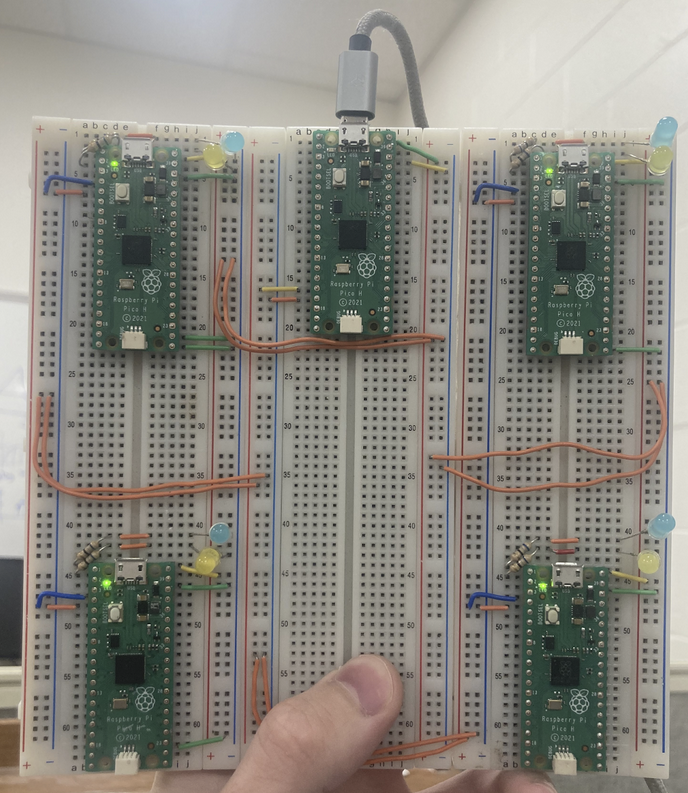
\includegraphics[width=\linewidth]{pico cluster.png}
\caption{The PentaPico Cluster.}
\label{pentapico_figure}
\end{figure}

% powering
All Picos are powered with $5$~V by a personal computer over the micro USB connection.
The USB~1.1 standard can support up to $2$~A of continuous current draw.
According to the Pico datasheet~\cite{picodocs:rpi}, the mean maximum VBUS current draw under a heavy workload is around $93.5$~mA at room temperature. 
This means that even if all Picos in the cluster are consuming their maximum power, the total consumption of the cluster remains well within the supported range.

% data connection
All Picos are connected by a single I$^2$C bus, allowing them to communicate with each other. 

% status LEDs
Each compute node has external blue and yellow status LEDs connected to GPIO pins $0$ and $1$ respectively via a $68\Omega$ current limiting resistor.
These complement the onboard status LED to allow for the cluster code to display its state in more depth, and were extremely helpful in debugging the software.

\section{Software}
\label{software_sec}
% (a) Programming Language: Which one did you use? Why?
% (b) Any reliability issues? What would happen in face of a hardware/software error?
% (c) Also list the versions for the operating system and other software. This is useful if anyone tries to reproduce this work down the road.

In this section I cover the software used in this project.
This includes the client program that serves as a user interface for sending image convolution jobs to the cluster and receiving results, as well as the programs on the head node and compute nodes of the cluster.

\subsection{Client Program}

Because the PentaPico cluster has no display and no connected input devices, to control the cluster a client program (\texttt{client.py}) is run on a personal computer connected over USB~1.1 serial.
The client program is written in Python, and tested on Python~3.11.8. 
It depends on the libraries matplotlib~3.8.3 for rendering results, Pillow~9.5.0 and numpy~1.26.4 for manipulating images, and pyserial~3.1 for communicating with the head node Pico.

\texttt{client.py} is a command line tool that takes the path to an input image as input.
It then opens a serial connection to the head node Pico and transmits the image along with the convolution kernel.
Once the head node has responded with the result of the convolution, \texttt{client.py} renders the result computed by PentaPico alongside the original input image, the ground truth result as computed by Pillow, and the difference between the ground truth and the PentaPico results.
That display is shown in Figure~\ref{client_result_figure}.

\begin{figure}[ht]
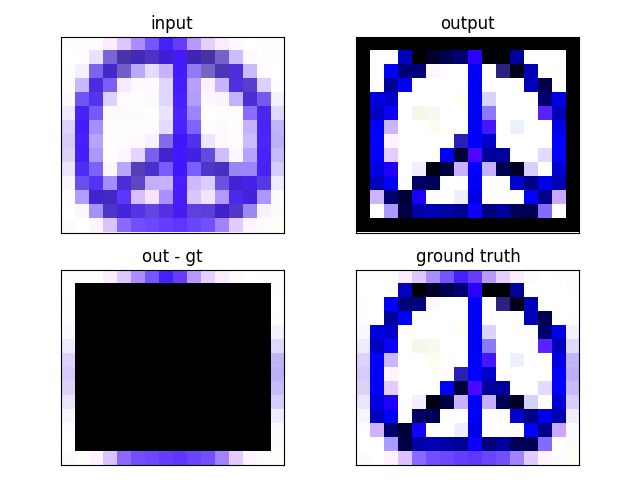
\includegraphics[width=\linewidth]{client.png}
\caption{The Result of a 3x3 sharpen filter convolved With the 14x16x3 ``peace.png'' image, as displayed by \texttt{client.py}.}
\label{client_result_figure}
\end{figure}

\texttt{client.py} is hardcoded to use a 3x3 sharpen filter, but the cluster can theoretically handle any filter  that is smaller than the input image itself.

\subsection{PentaPico Code}

The PentaPico code is written in C, compiled into a UF2 file with CMake~3.22.1, gcc~11.4.0, and uses the RPI Pico SDK version~2.1.1.
The code is split into two programs, one for the head node and one for the compute nodes.

\subsubsection{Head Node Code}
\label{head_node_sec}

The head node handles receiving jobs from \texttt{client.py} in the form of an image and convolution kernel, splitting the job among the four compute nodes, transmitting the job components to each compute node, and assembling the results to report back to \texttt{client.py}.

To limit the communication overhead, only the image data relevant to each compute node is transmitted to the compute nodes along with the necessary padding for the convolution kernel.
The image is sliced into rectangular sections via horizontal cuts based on the number of compute nodes in use for the job, where each slice contains enough padding to properly apply the convolution kernel.
When the job cannot be split perfectly evenly among each compute node, the last node receives a slightly larger job to ensure the entire image is convolved. 
Pseudoscope computing the slices of the image transmitted to each compute node is shown in Listing~\ref{split_listing}, where \texttt{total\_rows} is the height of the input image, and \texttt{row\_slice} and \texttt{row\_count} are used to decide which and how many rows to send to each compute node.

\begin{lstlisting}[
label=split_listing,caption=Data split pseudocode.]

int row_count, row_start;
for (i = 0; i<n_procs; i++) {
    // set start and row count to
    // include padding for the kernel
    row_start = (total_rows / n_procs)
                * i - (k_size/2);
    row_count = (total_rows / n_procs) 
                + (k_size-1);

    // handle the edge cases
    if (i == 0) {
        row_start = 0;
    } else if (i == n_procs-1) {
        row_count += k_size-1;
    }

    // .. transmit the slice ...
}
\end{lstlisting}

The result is that for the 14x16x3 \texttt{peace.png} image and $4$ compute nodes, nodes 0-2 get $5$ rows while node 3 gets $7$.

\subsubsection{Compute Node Code}
\label{compute_node_sec}
The compute nodes receive commands from the head node and process them. 
Each compute node is configured as an I$^2$C follower\footnote{I use ``leader/follower'' terminology in place of the old standard of ``master/slave''}, and sets its follower address to $23 + A_i$, where $A_i$ is the number represented by the binary state of GPIO pins $16$ and $17$.
When the I$^2$C bus is in use by the compute node, its external yellow status LED is lit.

If computations are performed in the I$^2C$ follower interrupt handler, the compute nodes will crash. 
Therefore, when a compute node receives a command from the head node it sets its global state based on that command.
The compute nodes operate in three states: \texttt{COMPUTE\_STATE\_IDLE}, \texttt{COMPUTE\_STATE\_ALLOCATE}, and \texttt{COMPUTE\_STATE\_CONVOLVE}.
In the main loop of the compute node, it performs different actions based on the state.

For \texttt{COMPUTE\_STATE\_IDLE}, the compute node flashes its on-board LED at a rate of $1$~Hz. This has the visual effect of keeping the LED lit, but reduces the brightness and power consumption of the LED.
While in \texttt{COMPUTE\_STATE\_ALLOCATE} or \texttt{COMPUTE\_STATE\_CONVOLVE}, the compute node sets its external blue status LED on.
In \texttt{COMPUTE\_STATE\_ALLOCATE}, the compute node allocates space for the job it is being asked to do and then changes its state to idle.
In \texttt{COMPUTE\_STATE\_CONVOLVE}, the compute node performs an image convolution on the slice of the image it has been given and then returns to idle.

When convolving, the algorithm used does not pad the input image.
This results in the output being cropped by a border of size $\frac{K_S-1}{2}$ on all edges, where $K_S$ is the side length of the convolution kernel.

\subsection{Overall Data Flow}

Due to the complexity of the data flow in the process of using the PentaPico cluster to compute an image convolution, the overall data flow is outlined in Figure~\ref{data_flow_figure}.

\begin{figure}[ht]
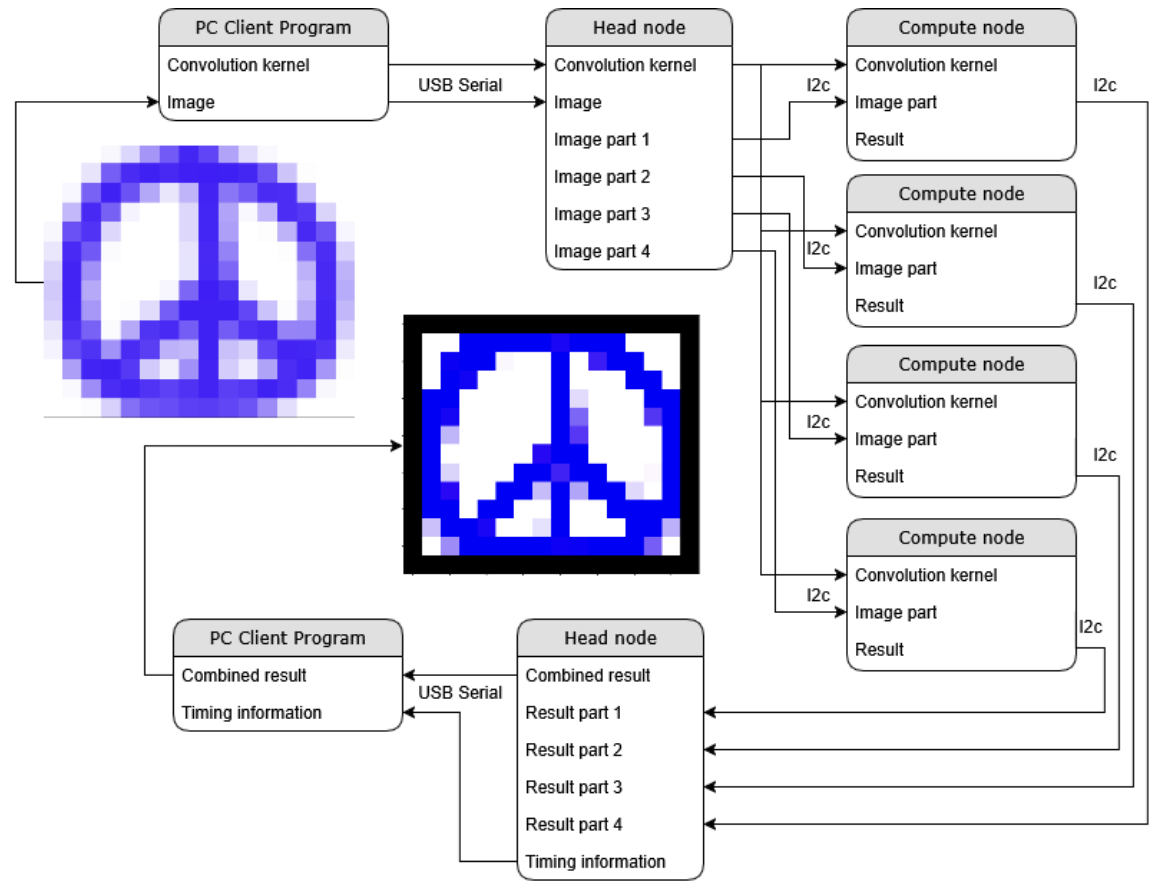
\includegraphics[width=8cm]{dataflow.png}
\caption{A high level overview of how data flows in the system.}
\label{data_flow_figure}
\end{figure}

% I have this figure in fuck-all nowhere so that it will be in a nicer spot for the rendered document
\begin{figure*}[ht]
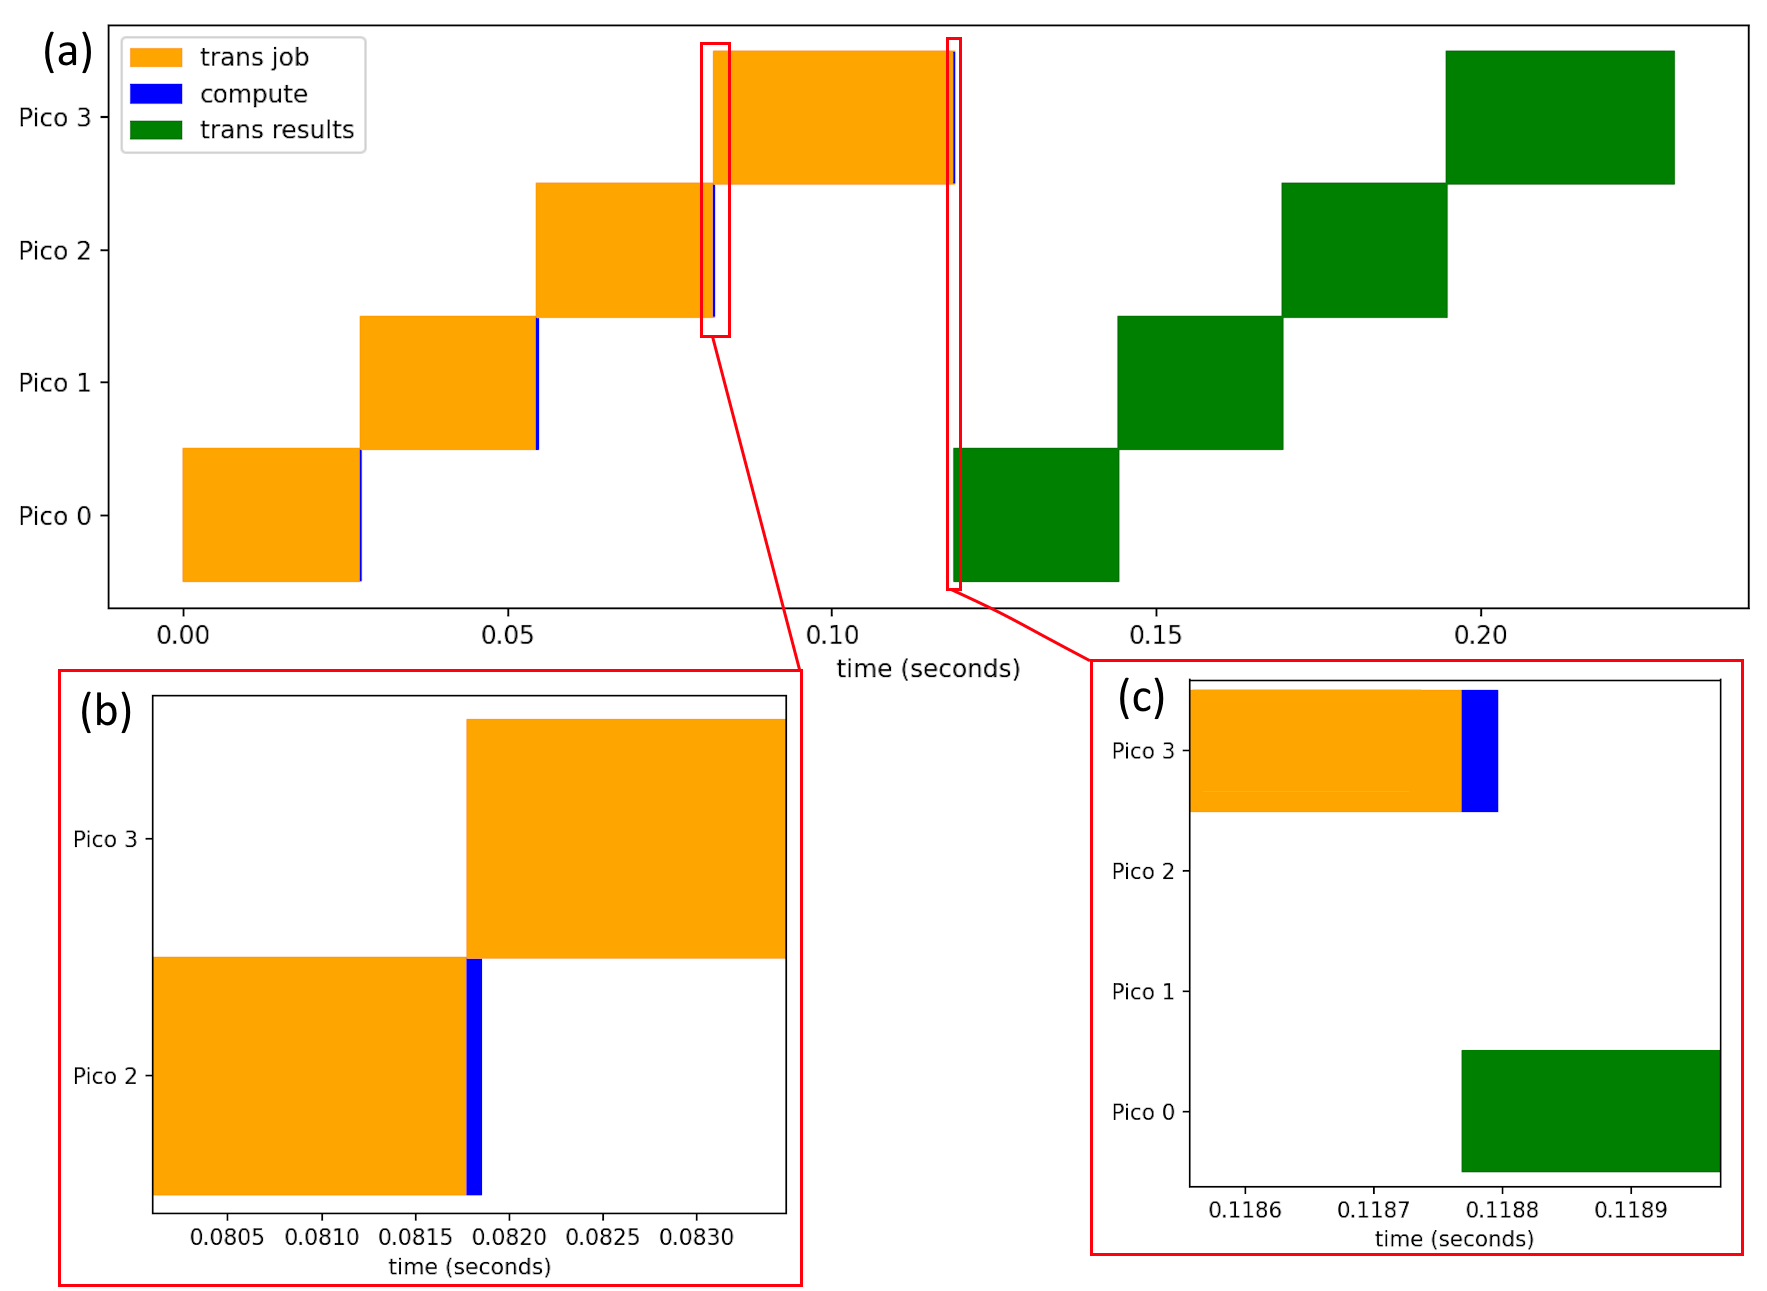
\includegraphics[width=\textwidth]{timeline_modified.png}
\caption{A reconstructed timing graph for the computation of a 3x3 convolution kernel over a 14x16x3 image using all four compute Picos showing (a) time spent transmitting the job to each pico, computing the job on each pico, and reading the results from each pico, (b) a zoomed in section of the timeline showing the transition from transmitting a job from one pico to another, and (c) a zoomed in section of the timeline showing the transition from transmitting and computing the jobs to retrieving the results.}
\label{timeline_plot}
\end{figure*}

Keep in mind that the figure does not represent any temporal information - I$^2$C communications cannot be performed in parallel. A more detailed view of the process of communicating between the head nodes and the compute nodes is shown in the following list, which accurately represents the serial nature of the I$^2$C communications:

\begin{enumerate}
    \item For each compute node:
    \begin{enumerate}
        \item Send kernel and image slice dimensions.
        \item Wait for compute node to allocate space.
    \end{enumerate}
    \item For each compute node:
    \begin{enumerate}
        \item Send kernel and image data.
    \end{enumerate}
    \item For each compute node:
    \begin{enumerate}
        \item Wait for the compute node to indicate it has complete its convolution.
        \item Read the results.
    \end{enumerate}
    \item Reassemble each convolved slice into an output image.
\end{enumerate}

How these communications play out in practice is discussed further in Section~\ref{results_sec}.

\subsection{Reliability Issues}
\label{reliability_sec}

% sometimes the cluster needs to be completely unpowered and repowered
The entire system has a few reliability issues. 
For one, on occasion the PentaPico gets stuck after completing a job and needs to be completely unpowered and repowered to reset it.

% sometimes the serial connection is really slow
Additionally, sometimes the serial connection between the personal computer and the head node hangs for a couple of seconds.
It is unclear to me whether this is an issue with the \texttt{client.py} Python code or the head node itself.

% sometimes it runs out of memory
Finally, since the Picos only have $256$~kB of SRAM, the head node can barely fit a 256x320x3 image stored as a character array along with a 3x3 convolution kernel in memory. 
This limits the potential problem space of the cluster severely when it comes to computing image convolutions.


\section{Project Overview and Results}
\label{results_sec}
% (a) Write about what you did.
% (b) Write about any results you obtained.
% (c) If your project involves performance, give time and power comparisons if possible.
% (d) Pictures and graphs are useful, if applicable.
% (e) Challenges: mention any difficulties or issues you had to overcome while working on the project

While I did successfully create a cluster that can compute image convolutions out of $5$ Picos, the cluster has remarkably terrible parallel efficicency.
To test this, with the cluster configured to use $1$, $2$, and $4$ compute nodes $N=10$ computations of the 3x3 sharpen filter convolved with the 14x16x3 \texttt{peace.png} image recorded and averaged.
The total head node time, speedup, and parallel efficiency are shown in Table~\ref{runtime_table}.
Total runtime (which includes the time spent transmitting information over USB serial) is omitted due to the inconsistencies mentioned in Section~\ref{reliability_sec}.

\begin{table}[tb]
\centering
\caption{Total runtime and head node runtime for the convolution of a 3x3 kernel over a 14x16x3 image for each Pico count, averaged over $N=10$ runs.}
\label{runtime_table}
\begin{tabular}{|c|c|c|c|c|}
\hline
\# Picos & Average head node runtime & Speedup & Parallel efficiency \\
\hline
\hline
$1$ & $183819\mu s$ & - & - \\
\hline
$2$ & $208807\mu s$ & $0.88$x & $0.44\%$ \\
\hline
$4$ & $241809\mu s$ & $0.76$x & $0.19\%$ \\
\hline
\end{tabular}
\end{table}

As seen in the table, using more Picos actually \textit{reduces} the performance of the cluster.
To explain why this is, a timing diagram is reconstructed for one of the runs in Figure~\ref{timeline_plot}.

The diagram shows the time each compute node spends receiving its slice of the job from the head node, computing the image convolution, and transmitting the results back to the head node.
The timing diagram shows two key issues with the PentaPico.
First, the time spent transmitting data is more than three orders of magnitude longer than that spent actually computing the image convolution.
Secondly, the only actual parallelism possible with the single-bus I$^2$C setup is that once a compute node has received its component of the job, it can perform its convolution while waiting for the bus to free up again.
All I$^2$C communications must happen in series, and since they take so much more time than the computations there is no performance benefit.

The average recorded runtime for each phase of computation is shown in Figure~\ref{nprocs_plot}.
It should be noted that for the ``4 Picos'' case, in each subplot the lower data point is actually three points stacked on top of each other. 
The outlier for that case is the last compute node, which receives a slightly larger problem size as mentioned in Section~\ref{head_node_sec}.

\begin{figure*}[ht]
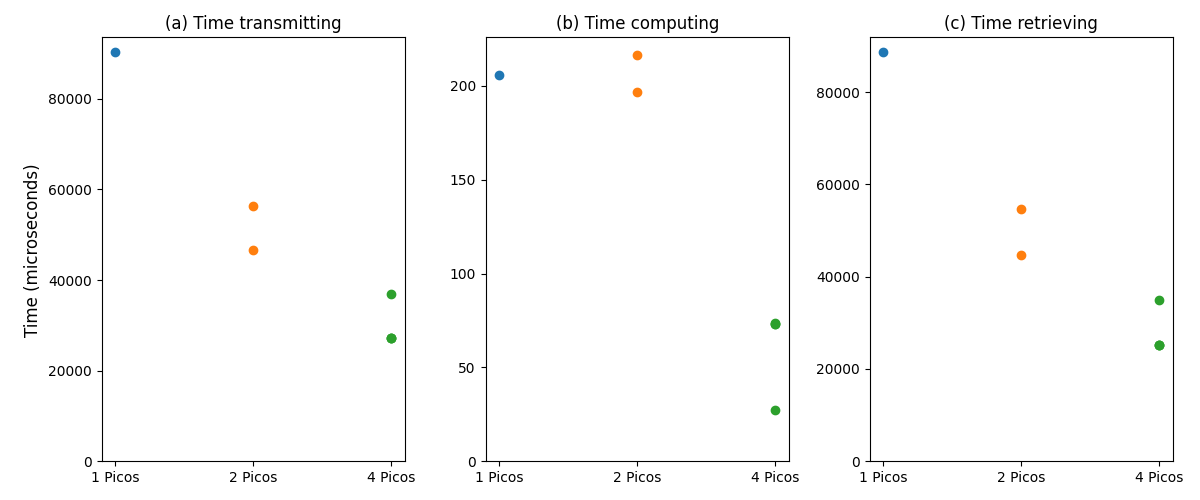
\includegraphics[width=\textwidth]{nprocs_plots.png}
\caption{Recorded runtime for (a) transmitting jobs from the head Pico to the compute Picos over I$^2$C, (b) computing the image convolution on each pico, and (c) retrieving the results from the compute Picos over I$^2$C for a 14x16x3 image and a 3x3 convolution kernel averaged over $N=10$ runs per Pico count.}
\label{nprocs_plot}
\end{figure*}

From the figure it can clearly be seen that as the number of compute nodes in use increases, the time spent communicating with or computing on each individual Pico drops.
However, as seen back in Table~\ref{runtime_table} the total time for each phase of computation actually increases.

The sole exception to this is the time spent computing for the $2$~Pico case. 
Even averaged over $10$ runs, the computation time for each node is very similar to that of the $1$~Pico case.
It is unclear to me what causes this, as the individual image slices are significantly smaller and should result in lower computation time.

\subsection{Challenges}

There were many obstacles and challenges encountered during this project. 
The most difficult challenge was certainly debugging. 
While I am able to easily print debug messages from the head node and transmit them over USB serial to see exactly what is happening in the head node, the same is not true for the compute nodes. 
Attempting to connect a second micro USB cable to one of the compute nodes while the cluster is powered on by the head node connection resulted in the connection to be lost, and may have risked damaging the Picos.
As such, to debug the compute nodes I created an artificial head node on each compute node that runs on the second core.
This artificial head node uses the second I$^2$C bus to send commands to the compute node's main core, and in this way the compute node can operate completely independently (and therefore take advantage of debugging over USB serial).

Another challenge was setting up the compute nodes to act as I$^2$C followers.
While the RPI Pico SDK does include some functions to assist setting this up, they are woefully under-documented.
Many core functions have absolutely no explanation of their purpose or function other than the name of the function, and this caused a lot of confusion when it came to setting up the compute nodes. 
There is furthermore a general lack of examples of using Picos as I$^2$C followers on the internet.
Fortunately, I was eventually able to figure it out based on code from Valentin Milea~\cite{i2c_slave}.

Finally, I was greatly limited by the small SRAM of the Picos. 
The implementation of the head node requires allocating an array for the input image as well as another array for the output image.
It is likely possible to get around this by using just one array for both the input and output, but this would require some very clever juggling of data that I was not comfortable messing with for this project.
The result is that while the Picos do have $256$~kB of SRAM, in practice the largest image size I can convolve is a little under $128$~kB --- that's barely enough for a 200x200x3 image.

\section{Conclusion}
\label{conclusion_sec}
% (a) Summarize what you did.
% (b) Future Work: List any improvements you might make if you had more time and resources to work on the project.

For my project I created a cluster computer out of five RPi Pico microcontrollers, consisting of one head node and four compute nodes.
The nodes communicate among each other over I$2$C, and the head node communicates with a client personal computer over USB~1.1 serial.
The cluster is programmed to compute image convolutions.
Although image convolution is an embarrassingly parallel task, the cluster is unable to achieve any speedup with multiple compute nodes in use, and had terrible parallel efficiency due to the extreme communication overhead required to transmit chunks of the job between the compute nodes.

Based on the results I see here, it seems likely to me that the reasoning people have for not using microcontrollers for cluster computing is that they are simply too limited. 
Microncontrollers in general do not have much memory and storage, and are not fitted to communicate via more methods like Ethernet.
Additionally, they are not designed to run contemporary operating systems like Linux.
This limits the breadth and depth of software that can be executed on a microcontroller cluster.
For example, on a cluster made of Raspberry Pi 4 single board computers, it is simple to run Linux on each node, communicate using a proper network, and execute common high performance computing benchmarks like HPL~\cite{petitet+:url17}.
However, on a microcontroller cluster one is generally limited to extremely light-weight operating systems at best, or forced to write bare metal code.
This may be in the process of changing --- Taube and Thiele~\cite{pico2:linux} have managed to get a lightweight Linux distribution running on the more recent Raspberry Pi Pico 2, but as it stands it seems unlikely that anything like running HPL on a microcontroller cluster is in reach.

For future work, it would be good to investigate different methods of transmitting data between the microcontrollers. 
For example, the Pico's custom PIO interface can theoretically sustain up to $360$~Mbps~\cite{2040docs:rpi}, while the Pico only supports up to $1$~Mbps for I$^2$C --- utilizing PIO could lead to a massive speedup.
It would also be interesting to develop a microcontroller cluster that makes use of a lightweight operating system like FreeRTOS in order to allow the cluster to run more general programs.



\bibliographystyle{IEEEtran}
\bibliography{bibliography.bib}

\end{document}
